\documentclass[epic,eepic,aspectratio=169,12pt]{beamer}
\usepackage[polish]{babel}
\usepackage[T1]{polski}
\usepackage[utf8]{inputenc}
\usepackage[T1]{fontenc}
\usepackage{color}
\usepackage{picture}
\usepackage{graphicx}
\usepackage{minibox}
\usepackage{csquotes}
%\usetheme{Copenhagen}
\usecolortheme{crane}

\usepackage[]{csquotes}
\DeclareQuoteAlias{german}{polish}
\usepackage[%style=numeric %,authoryear,  alphabetic, authoryear, ect.
sorting=nty,
isbn=true,
backend=biber]{biblatex}

\title{Discovery Service}

\setbeamertemplate{bibliography item}{\insertbiblabel}

\author{Krzysztof Pobożan}

\addbibresource{discoveryservice.bib}

\begin{document}
	\begin{frame}
		\maketitle
	\end{frame}
	\begin{frame}{Agenda}
		\tableofcontents
	\end{frame}
	\section{Wstęp}
	\begin{frame}{Gdzie uruchamiamy?}
		Czy głównym problemem infrastruktury jest elastyczność i odporność na awarię sieci.
		Jeśli uruchamiamy w chmurze jak AWS czy Azure to pewne awarie w małej skali są nieuniknione.
	\end{frame}
	\begin{frame}{CAP}
		\begin{description}
			\item[Consistent] spójność danych
			\item[Partition] rozproszenie/rozdrobnienie
			\item[Aviability] dostępność
		\end{description}
		Systemy bazodanowe rozproszone nie są wstanie spełnić wszystkich elementów CAP na raz.
	\end{frame}
	\section{Zookeeper Discovery Service}
	\begin{frame}{Zookeeper Discovery Service}
		Zookeeper jest złym rozwiązaniem dla Discovery Service uruchamianym na chmurze.
		Przekłada spójność danych nad dostępność.
		Dla koordynacji to jest dobre, jednak dla discovery service, lepiej mieć informacje częściowo fałszywe niż nie mieć żadnych informacji.
		
	\end{frame}
	\section{Eureka}
	\begin{frame}{Czym jest EUREKA}
		Serwis bazujący na REST do lokalizacji usług w celu równoważenia i zapobiegania utraty dostępu.\\
		Zaprojektowany do pracy w AWS.\\
		Głównym modułem jest \textbf{Eureka Serwer}, Netflix dostrcza również \textbf{Eureka Client} z prostym loadbalancigiem typu round-rubin.
	\end{frame}
	\begin{frame}{Jak działa Eureka?}
		\begin{figure}
			\centering
			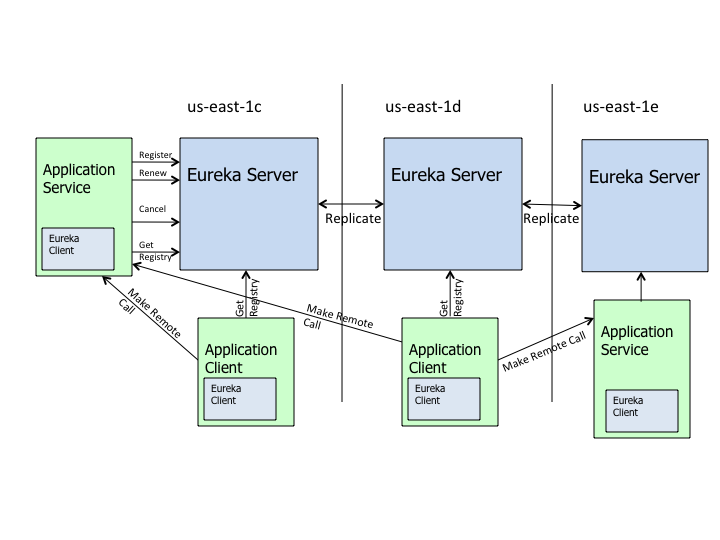
\includegraphics[width=0.6\linewidth]{eureka_architecture}
			\caption{Architektura usługi Eureka}
			\label{fig:eureka_architecture}
			\end{figure}

	\end{frame}
	\begin{frame}{Co daje spring-cloud?}
		\begin{itemize}
			\item Usługi rejestrowane są pod nazwą jak właściwość:  spring.application.name
			\item Proste uruchomienie swoich serwerów eureka
			\item Proste uzycie klienta - annotacja
			\item Wsparcie w RestTemplate dla eureki - w urlu wystarczy posłużyć się nazwą serwisu zamiast nazwy hosta.
		\end{itemize}
	\end{frame}
	\section{DEMO}
	\begin{frame}{DEMO}
		\href{https://github.com/krzpob/sample-eureka}{Przykład użyty w demo}
	\end{frame}
	\nocite{multi-zone}
	\nocite{netflix:eureka}
	\begin{frame}{Bibliografia}
		\printbibliography
	\end{frame}
\end{document}